
%%%%%%%%%%%%%%%%%%%%%%%%%%%%%%%%%%%%%%%%%%%%%%%%%%%%%%%%%%%%%
\subsubsection{模型建立}

针对问题二，本节从需求预测、成本定价和随机优化三个层面建立模型。

\textbf{步骤1：Prophet时序分解}

对每个品类的日销售量序列$S_{i,t}$，采用Prophet模型分解：
\begin{equation}
  S_{i,t} = g_i(t) + s_i(t) + h_i(t) + \varepsilon_{i,t}
\end{equation}
其中$g_i(t)$为趋势项（分段线性），$s_i(t)$为周期项（傅里叶级数，周+年），$h_i(t)$为中国节假日效应（含法定假日及调休窗口），$\varepsilon_{i,t}$为残差。

\textbf{步骤2：成本加成定价}

定价采用成本加成方法，加成率$\alpha_{i,t} \geq 0$为决策变量：
\begin{equation}
  P_{i,t} = (1 + \alpha_{i,t}) \cdot C_{i,t}
\end{equation}
有效单位成本计入损耗：
\begin{equation}
  C_{i,t}^{\text{eff}} = \frac{C_{i,t}}{1 - L_i}
\end{equation}

\textbf{步骤3：报童模型}

对每个品类$i$和日期$t$，单日期望利润为：
\begin{equation}
  \pi_i(Q, \alpha) = P \cdot \mathbb{E}[\min(Q, D)] + kP \cdot \mathbb{E}[(Q - D)^+] - C_i^{\text{eff}} \cdot Q
\end{equation}
其中$P = (1+\alpha)C_i$。第一项为正价销售收入，第二项为未售出商品按折扣价$kP$清仓的收入，第三项为含损耗的进货总成本。$k=0.66$为从打折数据估算的折扣价与正价比值的中位数。

需求$D$采用Prophet预测值$\hat{D}_{i,t}$经价格弹性调整：
\begin{equation}
  D_i(\alpha) = \hat{D}_{i,\text{Jul1}} \cdot \left(\frac{(1+\alpha)C_i}{(1+\bar{\alpha}_i)C_i}\right)^{e_i}
\end{equation}
需求分布采用Prophet残差的经验分布（非参数分位数），以Bootstrap重抽样计算期望利润。

\textbf{步骤4：约束与求解}

优化问题为$\max_{\alpha \geq 0,\; 0 \leq Q \leq Q_{\max}} \pi_i(Q, \alpha)$，其中$Q_{\max} = 1.5 \times \max_\tau S_{i,\tau}$为订货量上限。求解采用二维网格搜索（加成率35步$\times$订货量因子35步），每点5000次Monte Carlo抽样。

\subsubsection{模型求解}

基于上述模型，本节利用Python（Prophet, scipy）进行求解。Prophet在2023年5月31日前数据训练，预测31天至7月1日，2023年6月（30天）作为留出集评估。

各品类RMSE为7.7--34.1 kg，在全部六个品类上均优于ARIMA baseline（如花叶类34.1 vs 45.0 kg）。以花叶类为例，Prophet分解结果如图\ref{fig:prophet}所示。

\begin{figure}[H]
  \centering
  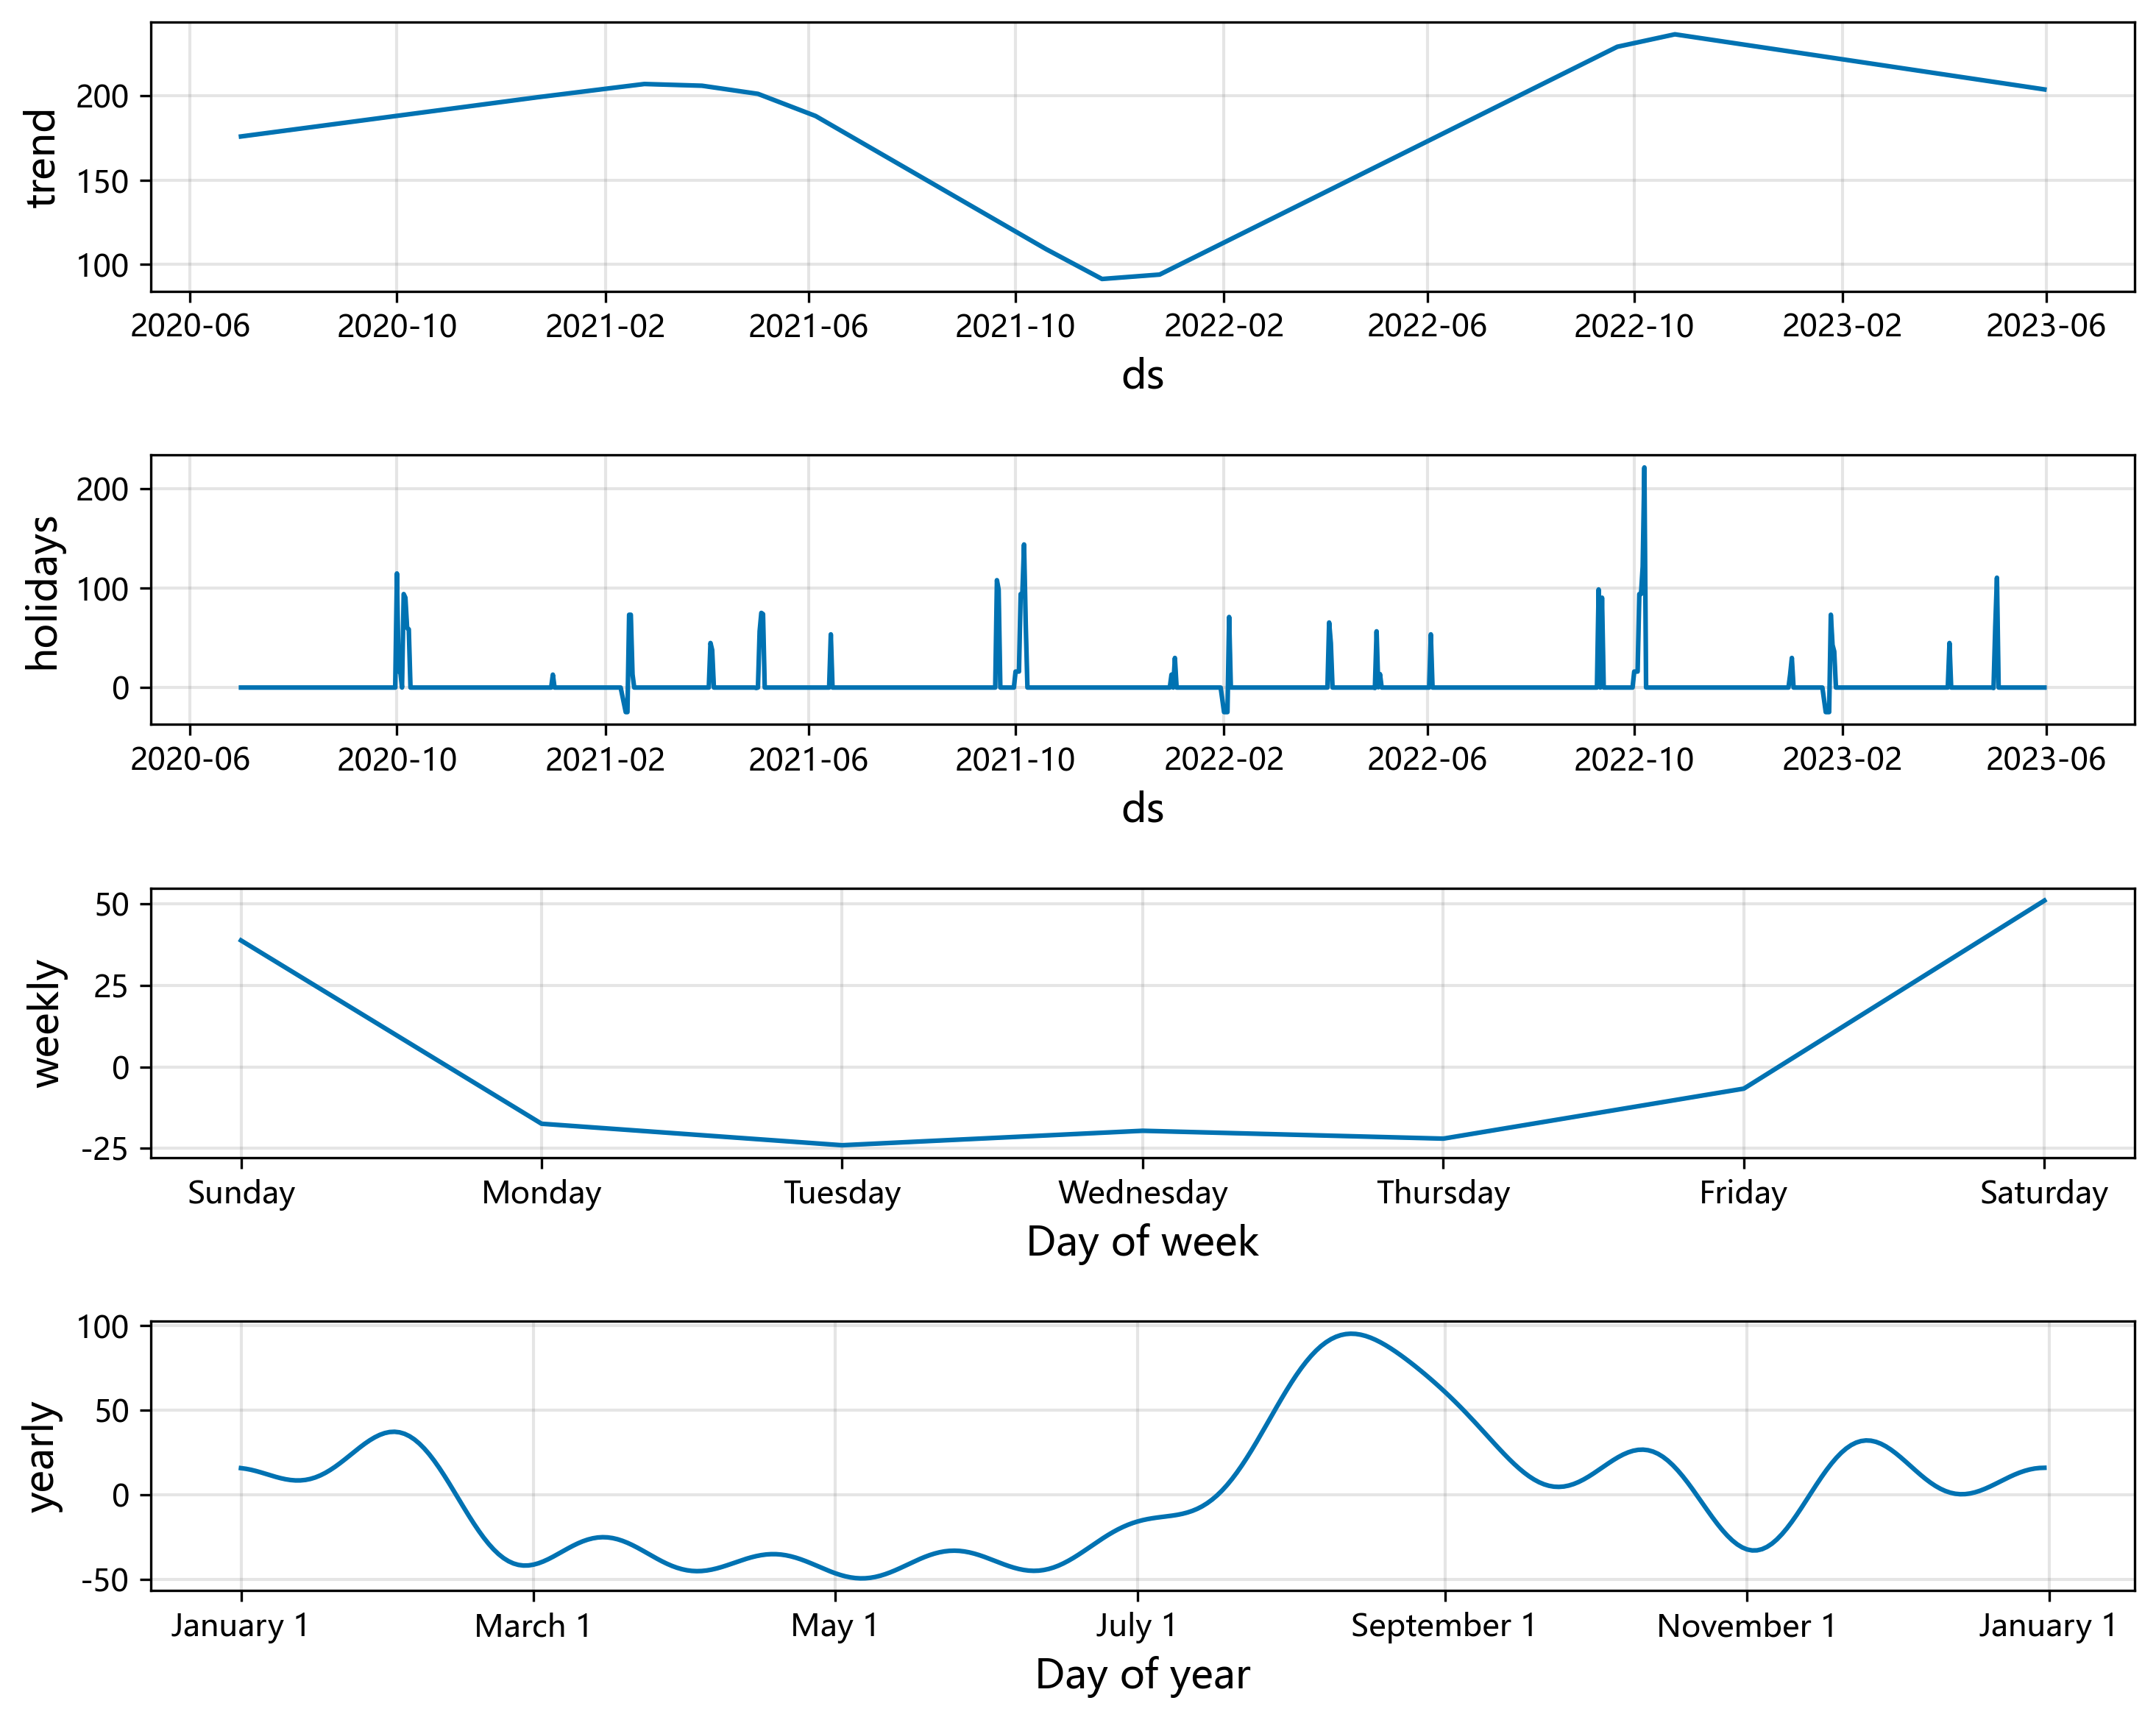
\includegraphics[width=0.90\textwidth]{figures/fig3_prophet_components.png}
  \caption{花叶类Prophet时间序列分解（趋势+周周期+年周期+节假日）}
  \label{fig:prophet}
\end{figure}

各品类2023年7月1日的最优策略如表\ref{tab:q2optimal}所示。

\begin{table}[H]
  \centering
  \caption{各品类最优补货与定价策略（2023年7月1日）}
  \label{tab:q2optimal}
  \begin{tabularx}{\textwidth}{CCCCC}
    \toprule
    品类 & 优化加成率 & 售价（元/kg） & 订货量（kg） & 期望利润（元） \\
    \midrule
    水生根茎类 & 103.6\% & 24.51 & 54.7 & 287 \\
    花叶类 & 116.7\% & 6.46 & 254.3 & 854 \\
    花菜类 & 104.6\% & 22.82 & 79.3 & 316 \\
    茄类 & 113.2\% & 20.04 & 53.3 & 162 \\
    辣椒类 & 128.2\% & 18.21 & 183.5 & 699 \\
    食用菌 & 113.0\% & 10.12 & 174.6 & 599 \\
    \midrule
    合计 & -- & -- & -- & \textbf{2918} \\
    \bottomrule
  \end{tabularx}
\end{table}

优化加成率（103.6\%--128.2\%）系统性高于历史均值（53.6\%--78.2\%），品类间有充分区分度（标准差0.082）。图\ref{fig:markup}展示了优化与历史的对比。

\begin{figure}[H]
  \centering
  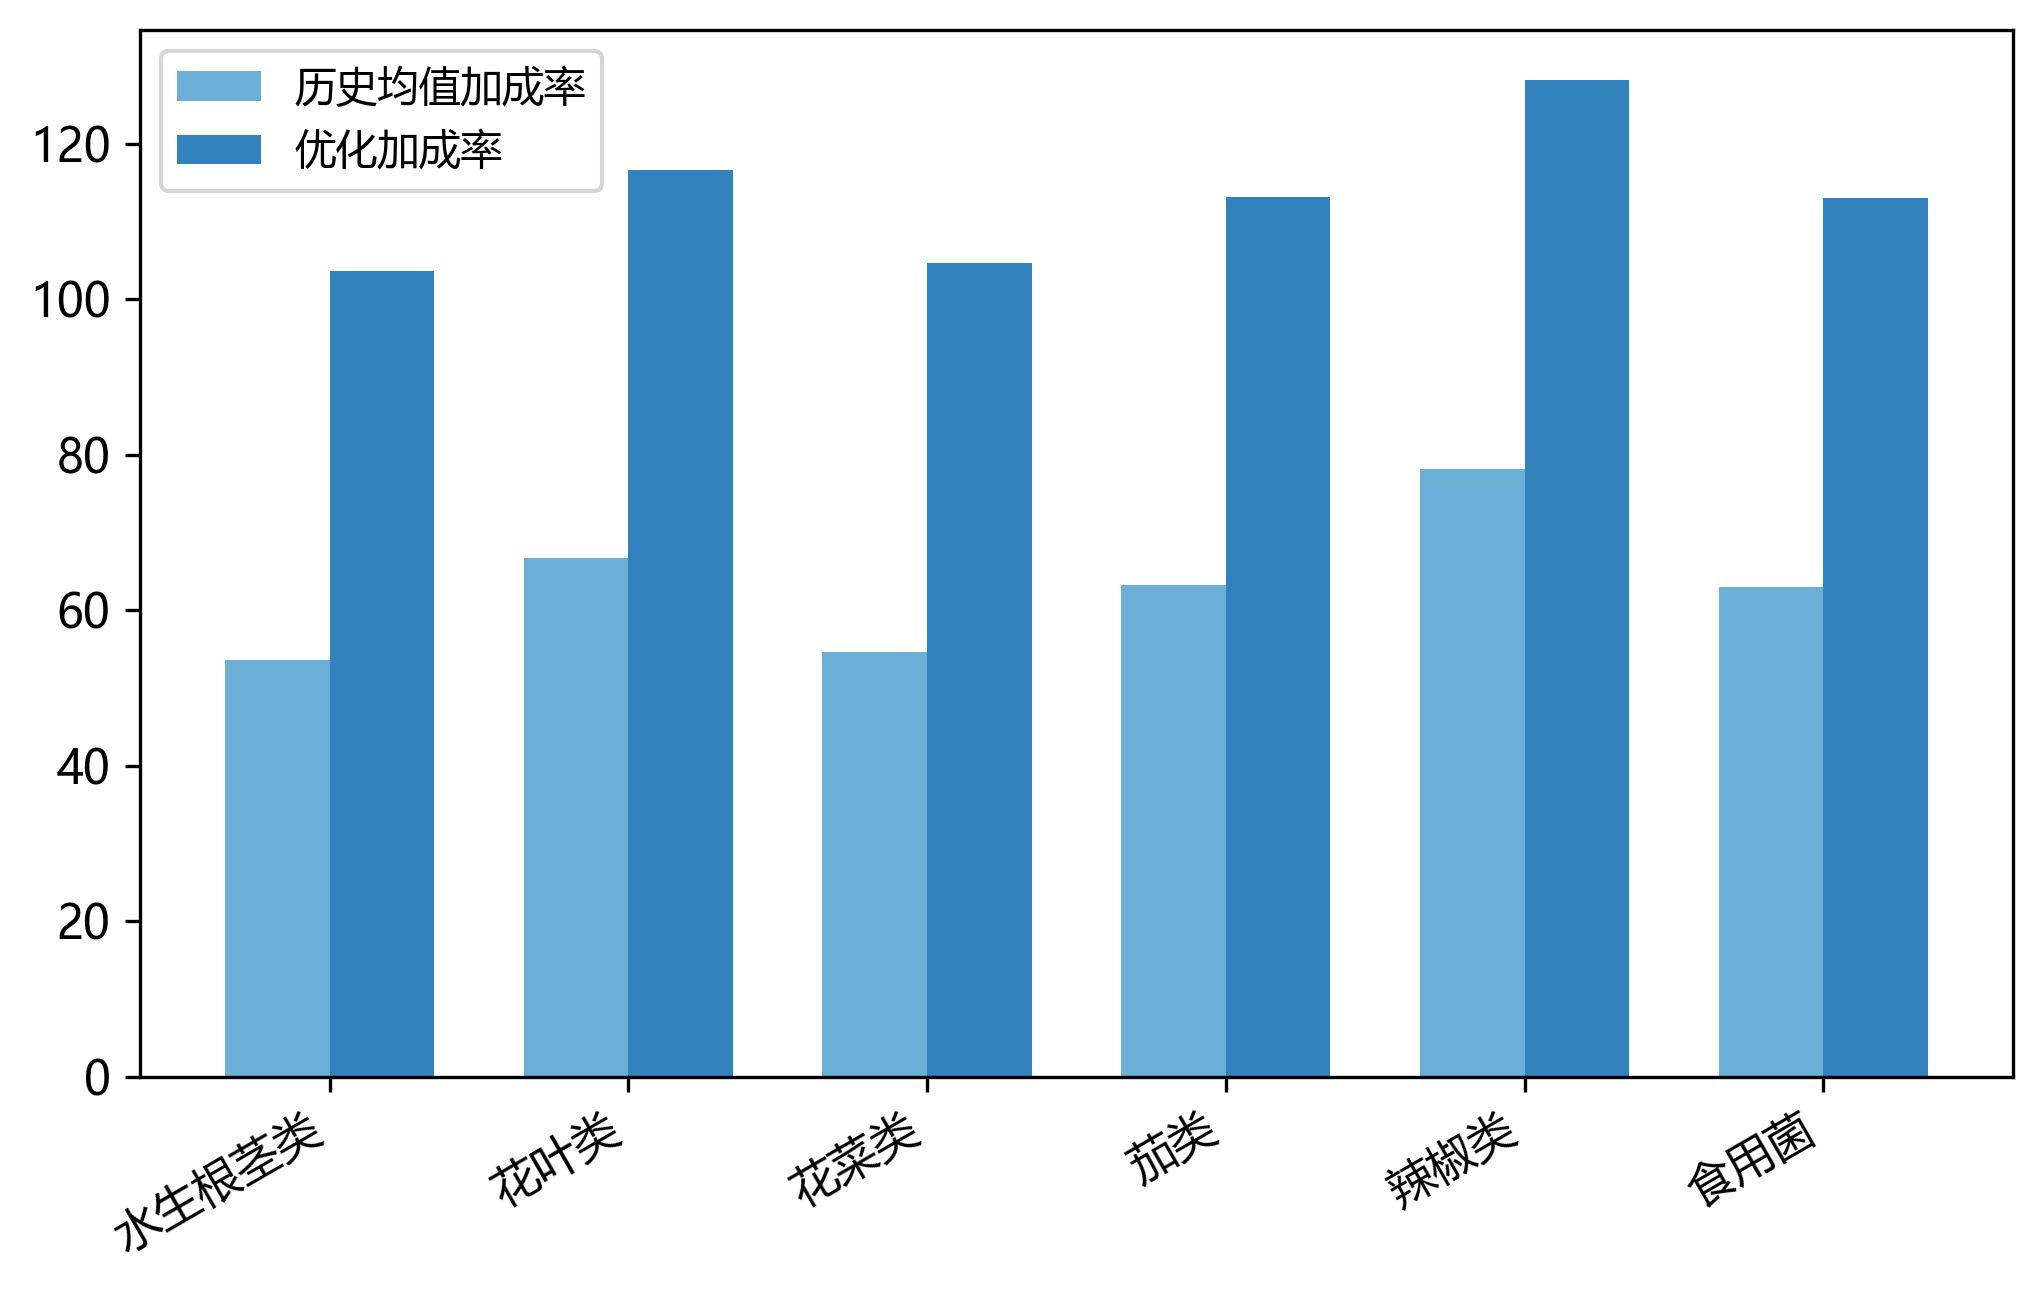
\includegraphics[width=0.80\textwidth]{figures/fig4_markup_comparison.png}
  \caption{各品类历史vs优化加成率对比}
  \label{fig:markup}
\end{figure}

设置ARIMA+固定加成baseline：以ARIMA替代Prophet，加成率固定为历史均值，订货量$Q = \hat{D}^{\text{ARISM}} / (1-L)$。相同利润函数和参数下，Baseline单日总利润为723元。M1增益（+304\%）来自两方面：Prophet更准确的季节性预测（如ARIMA将水生根茎类预测为$13.4$ kg而Prophet预测$30.6$ kg），以及加成率优化。

对7月2--7日，每日基于Prophet向前一步预测，以当日最新批发价重新运行报童优化，每日独立决策。七日总期望利润为20427元（$k=0.66$），系七日独立优化利润之和。为评估$k$的不确定性影响，对$k\in[0.50,0.75]$各值重新运行完整的二维网格搜索求解最优$(Q,\alpha)$，得到七日利润区间$[16534,\; 25991]$元。该区间非对称于$k=0.66$（偏向下限），原因在于$k$降低时残值回收锐减，迫使系统削减订货量而利润下降更快；$k$升高时订货量增加但受需求上限$Q_{\max}$约束，利润增益边际递减。这一处理假设每日进货决策仅依赖当日预测，不考虑前日剩余库存（题目假设当日未售出隔日无法销售，自然满足）和未来多日需求关联。

Prophet在所有六个品类上的留出集RMSE为7.7--34.1 kg，约束报童模型给出了103.6%--128.2%的差异化加成率。M1相较ARIMA+固定加成baseline的304%增益中，Prophet的季节性预测贡献了主要的精度提升，加成率优化贡献了额外的利润空间。
